
\section{$m$-Correlation Clustering on General Graphs}

% \subsection{Correlation Clustering IP}

% If $u,v$ are in the same cluster, $x_{uv} = 0$. Else $x_{uv} = 1$.

% \begin{alignat}{3} \label{IP:CC}
% 		&\text{Find: } && \argmin\ \sum_{(u,v) \in E^+} x_{uv} + \sum_{(u,v) \in E^-} (1- x_{uv}), \nonumber\\
% 		&\text{Subject to:} \quad && \forall u,v,w,\ x_{uv} \le x_{uw} + x_{vw}, \nonumber\\
% 		& && \forall u,v \in [n],\ x_{uv} \in \{ 0,1 \}.\tag{IP1}
% \end{alignat}

% \subsection{Problem 3}

% Find the minimum number of points to remove, such that the optimal correlation clustering has value $0$.
% \begin{alignat}{3} \label{IP:CC3}
% 		&\text{Find: } && \argmin\ \sum_{u \in [n]} Y_u, \nonumber\\
% 		&\text{Subject to:} \quad && \forall u,v,w,\ x_{uv} \le x_{uw} + x_{vw}, \nonumber\\
% 		& && \forall (u,v) \in E^+,\ Y_u + Y_v \ge x_{uv}, \nonumber\\
% 		& && \forall (u,v) \in E^-,\ Y_u + Y_v \ge 1 - x_{uv}, \nonumber\\
% 		& && \forall u,v \in [n],\ x_{uv} \in \{ 0,1 \},\nonumber\\
% 		& && \forall u \in [n],\ Y_u \in \{ 0,1 \}. \tag{IP2}
% \end{alignat}

% \subsection{$m$-robust correlation clustering}

% Find the optimal correlation clustering after being allowed to remove at most $m$ vertices.
% \begin{alignat}{3} \label{IP:CC4}
% 		&\text{Find: } && \argmin \sum_{(u,v) \in E} z_{uv}, \nonumber\\
% 		&\text{Subject to:} \quad && \forall u,v,w,\ x_{uv} \le x_{uw} + x_{vw}, \nonumber\\
% 		& && \forall (u,v) \in E^+,\ Y_u + Y_v + z_{uv} \ge x_{uv}, \nonumber\\
% 		& && \forall (u,v) \in E^-,\ Y_u + Y_v + z_{uv} \ge 1 - x_{uv}, \nonumber\\
% 		& && \sum_{u} Y_u \le m \nonumber \\
% 		& && \forall u,v \in [n],\ x_{uv} \in \{ 0,1 \},\nonumber\\
% 		& && \forall u,v \in [n],\ z_{uv} \in \{ 0,1 \},\nonumber\\
% 		& && \forall u \in [n],\ Y_u \in \{ 0,1 \}. \tag{IP3}
% \end{alignat}

\begin{theorem}[reference] \label{theorem:clustering:1}
For any metric space $(X,d)$ and parameter $\Delta$, there exists a distribution over clusterings such that for any two points $u,v \in X$, any clustering $\mathcal{C}$ with non-zero probability satisfies:
\begin{align*}
\forall C \in \mathcal{C},\ \mathrm{diam} (C) &\le \Delta \nonumber\\
\prob (u,v \text{ are in different clusters}) &\le \frac{d(u,v)}{\Delta} \mathcal{O} \left( \log{n} \right). \nonumber
\end{align*}
\end{theorem}

\begin{theorem}[reference] \label{theorem:clustering:2}
For any metric space $(X,d)$ and parameter $\Delta > 0$, {\sf PaddedCluster}$(V,\mathbf{x},\Delta)$ outputs a randomized clustering of $X$ such that:
\begin{align*}
\forall C \in \mathcal{C},\ \mathrm{diam} (C) &\le \Delta \nonumber\\
\prob (\mathrm{Ball}_\rho(x)\nsubseteq \mathcal{C}(x)) &\le \alpha (x) \frac{\rho}{\Delta}.\nonumber
\end{align*}
where $\alpha(x) = \mathcal{O}( \log (\frac{|B_{\Delta}(x)|}{|B_{\Delta/8}(x)|}) ) = \mathcal{O} (\log n)$ and $\mathcal{C} (x)$ indicates the set of points in the same cluster as $x$.
% \begin{enumerate}
%     \item Each cluster $C$ in $P$ has diameter at most $\Delta$.
%     \item For every $x\in X$ and $\rho>0$
%     \begin{align*}
%         \prob (B_\rho(x)\nsubseteq \mathcal{C}(x)) \leq \alpha(x)\frac{\rho}{\Delta}
%     \end{align*}
%     where $\alpha(x)=O ( \log (\frac{|B_{\Delta}(x)|}{|B_{\Delta/8}(x)|}) ) $
% \end{enumerate}
\end{theorem}

\begin{algorithm}
\caption{{\sf PaddedCluster}$(V,\mathbf{x},\Delta)$}
\label{alg:cluster}
\begin{algorithmic}[1]
\Statex \textbf{Input:} A metric space $\mathbf{x}$ on a set of points $V$ \Comment{$\mathbf{x}_{uv}$ is the distance between $u,v$}
\Statex \textbf{Output:} A clustering of $V$ with properties as stated in Theorem \ref{theorem:clustering:2}
\State Fix an $r^* \in [\Delta/4, \Delta/2]$ chosen uniformly at random.
\State Pick a uniformly random permutation of points in $V$, denoted $\sigma$
\While {$V_{uc} \ne \phi$}
\State $C \gets \{ u \in V_{uc} : x_{uv} \le r^* \}$
\Comment{Unclustered points within distance $r^*$ of $v$}
\State $V_{uc} \gets V_{uc} \setminus C$ \Comment{Remove newly clustered vertices}
\State Augment $\mathcal{C}$ by $C$
\EndWhile
\Statex \textbf{Return:} $\mathcal{C}$
\end{algorithmic}
\end{algorithm}



% The clustering is as follows:
% \begin{enumerate}
% \item Fix an $r^* \in [0,\Delta/2]$ uniformly chosen from this set.
% \item Pick a random permutation of points in $X$, called $\sigma$.
% \item Iterate over points in $\sigma$ and for the $i^{th}$ point, form a ball of radius $r^*$ around this and allocate the points that have not yet been allocated to any point to this cluster. Iterate until no unclustered point remains.
% \end{enumerate}

{\color{red}
\begin{proof}
\begin{figure}[ht]
\centering
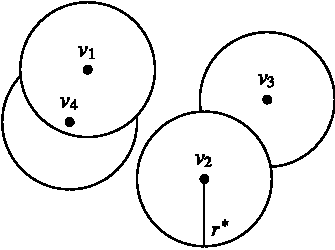
\includegraphics{./img/rand-clustering.pdf}
\caption{Clustering in Theorem \ref{theorem:clustering:1}}
\label{fig:3}
\end{figure}

The proof of Theorem \ref{theorem:clustering:1} is as follows:
\begin{description}
	\item[Bounded diameter] Consider two points $u$ and $v$. Since $r^*$ is fixed to be between $0$ and $\Delta / 2$, then if the two points belong in the same cluster, they must both be within a distance of $r^*$ of some point $v$. Therefore, by the triangle inequality for the metric $\mathbf{x}$ they are not separated by a distance more than $\Delta$. Therefore, the diameter of each cluster is at most $\Delta$.
	\item[Probability of separating points] Consider any two points $u$ and $v$. A vertex $w$ is said to \textit{settle} the pair $(u,v)$ if it is the first vertex in the order specified by $\sigma$ such that at least one of $u$ and $v$ belong to the $r^*$-ball centered at $w$. For every pair of points $(u,v)$, $u$ or $v$ itself is a possible candidate for the settling vertex, so at least one settling vertex must exist.
	Let $L_{uv}$ represent the set of vertices which include at least one of $u$ and $v$ lie in the $r^*$-ball centered at $w_i$. Let $\pi_{uv}$ denote vertices ordered as per the minimum of their distances to $u$ and $v$. Then, for some $k$, the set $L_{uv}$ will include the first $k$ vertices of $\pi_{uv}$ and not include the remaining vertices. For a particular $w$, the probability that it settles $(u,v)$ is equal to the probability that $w \in L_{uv}$ and $w$ is first among the vertices of $L_{uv}$. If $w$ is in $L_{uv}$, then all vertices before $w \in \pi_{uv}$ must belong to $L_{uv}$. Therefore, the probability that $w_i$, the $i^{th}$ vertex in $\pi_{uv}$ settles $(u,v)$, satisfies, for fixed radius $r^*$,
	\begin{equation*}
		P (w_i \text{ settles } (u,v) | r^*) = \frac{1}{L_{uv}} \le \frac{1}{i}
	\end{equation*}
	Therefore, the probability that $u$ and $v$ are separated into different clusters (cut) is equal to:
	\begin{align}
		P (u,v \text{ lie in different clusters}) &= \mathbb{E}_{r^*} \left[\sum_{w_i \in \pi} P (w \text{ cuts } (u,v) | r^*) \right] \\
		&= \mathbb{E}_{r^*} \left[\sum_{w_i \in \pi} P (w_i \text{ settles } (u,v) | r^*) \cdot P (w_i \text{ cuts } (u,v) | r^*, w_i \text{ settles } (u,v)) \right] \\
		&\overset{(i)}{\le} \sum_i \frac{1}{i} P( d(w_i,u) \le r^* \le d(w_i,v) ) \label{ineq:1}\\
		&= \sum_i \frac{1}{i} \frac{d(w_i,v) - P( d(w_i,u)}{0.5 \Delta} \\
		&\le \sum_i \frac{1}{i} \frac{d(u,v)}{0.5 \Delta} \\
		&= H_n  \frac{d(u,v)}{0.5 \Delta} \\
		&\le 2 \log{n} \frac{d(u,v)}{\Delta}
	\end{align}
\end{description}
\end{proof}}

\begin{comment}
\begin{theorem} \label{theorem:clustering:2}
Let $(X,d)$ be a metric space on n points, and $\Delta>0$. There is a probabilistic distribution of partitions $P$ of $X$ that satisfies the following properties:
\begin{enumerate}
    \item Each cluster $C$ in $P$ has diameter at most $\Delta$.
    \item For every $x\in X$ and $\rho>0$
    \begin{align*}
        Pr(B_\rho(x)\nsubseteq P(x)) \leq \alpha(x)\frac{\rho}{\Delta}
    \end{align*}
    where $\alpha(x)=O ( \log (\frac{|B_{\Delta}(x)|}{|B_{\Delta/8}(x)|}) ) $
\end{enumerate}

%The above clustering can be modified such that the probability that for every vertex $v$, the probability that it is cut by a ball of radius $\epsilon$ is proportional to $\epsilon$. In other words, smaller balls are more likely to lie entirely within a cluster than larger balls.
\end{theorem}
\begin{proof} {\color{red} [verify]}
The clustering is as follows:
\begin{enumerate}
\item Fix an $r \in [\Delta/4,\Delta/2]$ uniformly chosen from this set.
\item Pick a random permutation of points in $X$, called $\sigma$.
\item Iterate over points in $\sigma$ and for the $i^{th}$ point, form a ball of radius $r$ around this and allocate the points that have not yet been allocated to any point to this cluster. Iterate untill no unclustered point remains.
\end{enumerate}

We'll consider $\rho<\Delta/8$ otherwise the guarantees are trivial. Consider a point $x$. Sort vertices of $X$ w.r.t distance from $x$. Call the sequence $\pi=\{u_1,u_2,\dots,u_n\}$. Define $A_i=d(u_i,x)+\rho$ and $B_i=d(u_i,x)-\rho$. Clearly $A_1<A_2<A_3,\dots,A_n$ and $B_1<B_2<B_3,\dots,B_n$.\\
Now consider if $x\in B_r(u_i)$ but $B_{\rho}(x)\nsubseteq B_r(u_i)$, then
\begin{align*}
    r &\in [A_i + \rho,B_i) \\
    \implies r &\in [A_i,B_i)
\end{align*}
Let the event $\beta_i$ denote the event that $u_i$ is the first vertex such that $r\geq A_i$. If $\beta_i$ and $r\geq B_i$, then:
\begin{enumerate}
    \item $B_\rho(x)\cap B_r(u_j)=\phi$ for $\forall j<i$
    \item $B_\rho(x)\subseteq B_r(u_i)$
\end{enumerate}
Thus
\begin{align*}
    Pr(B_{\rho}(x)\nsubseteq P(x)) \leq \sum_{1\leq i\leq n}Pr(\beta_i \; and \; A_i\leq r < B_i)
\end{align*}

Note that $Pr(\beta_i|r)<\frac{1}{i}$ and $Pr(A_i\leq r < B_i) \leq \frac{B_i-A_i}{\Delta/4}=8\rho/\Delta$. Now if $\Delta/2<A_i$ then $r<A_i$ (because $r\in[\Delta/4,\Delta/2]$), and so $\beta_i$ won't happen. Also, if $i>|B_\Delta(X)|$ then $u_i\notin B_{\Delta}(x)$ (since all vertices $u_i$ are sorted according to their distance to $x$) and hence
\begin{align*}
    A_i=d(u_i,x)-\rho \geq \Delta-\rho > \Delta/2 
\end{align*}
We use the fact that $\rho<\Delta/2$. And hence $Pr(\beta_i)=0$. Additionally, if $\Delta/4>B_i$ then $r>B_i$ and $Pr(A_i \leq r < B_i)=0$. Therefore if $i\leq |B_{\Delta/8}|$ then $u_i\in B_{\Delta/8}(x)$ and $B_i=d(u_i,x)+\rho \leq \Delta/8+ \rho < \Delta/4$ and hence $Pr(A_i\leq r <B_i)=0$. We conclude that:
\begin{align*}
    Pr(B_\rho(x)\nsubseteq P(x)) \leq \sum_{i=|B_{\Delta/8}(x)|}^{|B_{\Delta}|}\frac{1}{i}\cdot \frac{8\rho}{\Delta} = O\left(\log\frac{|B_{\Delta}|}{|B_{\Delta/8}(x)|} \cdot \frac{8\rho}{ \Delta } \right)
\end{align*}

%I read the proof of this theorem and writing it down here
%The clustering can be changed to pick $r^*$ from $[\Delta/4, \Delta/2]$ instead of just $[0, \Delta]$.
\end{proof}

This will be used to give a rounding algorithm for Problem~\ref{IP:CC3}.

\begin{proposition}[A $\log^2 (n)$ approximation to \ref{IP:CC3}]
The algorithm is as follows:


\begin{enumerate}
    \item Solve the LP relaxation of \ref{IP:CC3} optimally and denote its solution $\{ x_{uv}^* : (u,v) \in \binom{V}{2} \} \cup \{ Y_u^* : u \in V \}$. Define $\hat{x}_{uv} = x_{uv}^* + n^{-2}$.
    \item Randomly cluster the points as per Theorem~\ref{theorem:clustering:2} (with distance between points given by $\hat{x}_{uv}$) and consider $V^-$, all vertices connected by negative edges that are placed in the same cluster.
    \item Consider the subgraph formed by $V^-$ and the corresponding unsatisfied negative edges.
    \item Find a $2$-approximate vertex cover on this subgraph. For every negative edge, at least one of its end points will be removed and the resultant vertices will have all negative edge constraints satisfied.
    \item Consider the remaining vertices in the graph. Among these vertices, unsatisfied constraints are only because of points separated by a positive edge being put into different clusters. Let these vertices be denoted $V^+$.
    \item Once again find a $2$-approximate vertex cover on the subgraph formed by $V^+$ and the corresponding unsatisfied positive edges. Remove these vertices from the graph.
    \item Return the remaining vertices in the graph. There exists a clustering of these vertices with $0$ cost.
\end{enumerate}
\end{proposition}
\begin{proof}
{\color{red} change the negative edge analysis to reflect the modification in the algorithm}
\begin{enumerate}
	\item The first step of the algorithm is to solve the LP optimally. Consider its solution $\{ x_{uv}^* : (u,v) \in \binom{[n]}{2} \} \cup \{ Y_u^* : u \in [n]\}$. Recall that $\hat{x}_{uv}$ is defined as $x_{uv}^* + n^{-2}$.
	\begin{observation} The set of distances $\{ \hat{x}_{uv} \}$ forms a metric. This is because all distances are incremented by the same quantity.
	\end{observation}
	\item Since the set $\{ \hat{x}_{uv} \}$ forms a metric, one may find a randomized clustering $C$ (over all vertices) according to Theorem~\ref{theorem:clustering:2} in such a way that the diameter of each cluster is $\le \Delta$ which is chosen as $0.25$. Let the clustering be denoted $c_{uv}$ ($=0$ if $u$ and $v$ are in the same cluster and $1$ otherwise). The property of the clustering solution is that if $\hat{x}_{uv}$ is high, then the points $u,v$ are likely to lie in different clusters while if they are in the same cluster, they cannot be too far apart. This will be useful in rounding the optimal solution.

	\item Consider the vertices $V^-$ which are connected to at least one unsatisfied negative edge constraint and consider the subgraph $G^-$ formed by $V^-$ and these unsatisfied negative edges. For every vertex $v \in V^-$, there exists at least one other vertex in $u \in V^-$ with a negative edge to $u$, having $c_{uv} = 0$. Therefore, for such edges, the constraint that must necessarily be satisfied is
	\begin{equation*}
        Y_u^* + Y_v^* \ge 1 - x^*_{uv}
	\end{equation*}
	By the clustering in Theorem~\ref{theorem:clustering:2}, two points in the same cluster are not separated by a distance of more than $\Delta = 0.25$. Therefore, $c_{uv} = 0 \implies \hat{x}_{uv} \le 0.25 \implies x_{uv}^* \le 0.25 - \frac{1}{n^2}$. Therefore, we must necessarily have:
	\begin{equation} \label{eq:001}
		Y_u^* + Y_v^* \ge 0.75 + \frac{1}{n^2} \ge 0.75
	\end{equation}
	In Step 3 of the algorithm, we compute a $2$-approximate vertex cover over $G^-$. We consider a standard algorithm for vertex cover which is $2$-approximate.

\begin{algorithm}
\caption{{\sf ApproxVC}$(G)$}
\label{alg:min-edge-uncover}
\begin{algorithmic}[1]
\State \textbf{Input:} A graph $G = (V,E)$
\State \text{Ouput:} Set of vertices which is a $2$-approximation for minimum vertex cover
\State \textbf{Initialization:} $E_{uc} = E$ \Comment{Set of uncovered edges}
\While{$E_{uc} \ne \phi$}
\State Choose an arbitrary $e = (u,v) \in E_{uc}$
\State $VC \gets VC \cup \{ u,v \}$ \Comment{Add both end-points of $e$ to the vertex cover}
\State $E_{uc} \gets E_{uc} \setminus \left( N(u) \cup N(v) \right)$ \Comment{Remove all edges covered by $u$ and $v$ from $E_{uc}$}
\EndWhile
\State \textbf{Return} $VC$
\end{algorithmic}
\end{algorithm}
	
	
% 	\begin{algorithm}[$2$-approximation for Vertex Cover] Pick an arbitrary negative edge constraint in this subgraph and discard both its end points. Choose any negative edge constraint that still remains unsatisfied and pick its end points. Repeat until no unsatisfied negative edge constraints remain.
% 	\end{algorithm}
	For each edge in $G^-$, define a random variable $a_e$ which is equal to $1$ if edge $e$ is chosen by the vertex cover algorithm and $0$ otherwise. Let $\opt_-$ denote the component of the optimal solution corresponding to vertices in $V^-$. By the optimality of $Y^*_u$ we have,
	\begin{align}
	\opt_- \ge \sum_{u \in V^-} Y^*_u &\ge \sum_{e = (u,v) \in G^-} (Y_{u}^* + Y_{v}^*) \cdot a_{e} \cdot c_{uv}, \nonumber\\
	&\overset{(i)}{\ge} \sum_{e = (u,v) \in G^-} 0.75 \cdot a_{e} \cdot c_{uv}. \label{eq:005}
	\end{align}
	where $(i)$ follows from Eq.~\eqref{eq:001}. On the other hand, the number of vertices removed by the algorithm in Step 4 is equal to twice the number of edges chosen in the vertex cover algorithm,
	\begin{equation*}
	\alg_- = \sum_{e = (u,v) \in E^-} 2 \cdot a_{e} \cdot c_{uv} \le \frac83 \opt_-.
	\end{equation*}
	where the last inequality follows from Eq.~\eqref{eq:005}. Therefore, among the set of vertices considered in Step 3 of the algorithm, the number of vertices discarded (in Step 4) is bounded by a constant fraction of the number of vertices discarded in the optimal solution.

% 	\item On the other hand, for positive edges, the situation is more precarious, but we will show that the same clustering (which is done for the entire metric) can be used to round effectively.
% 	For any positive edge, $(u,v) \in E^+$, $u$ and $v$ must belong in the same cluster for the cost of the clustering to be equal to $0$. They must also satisfy the constraint:
% 	\begin{equation} \label{eq:002}
% 		Y_u^* + Y_v^* \ge x_{uv}^*
% 	\end{equation}
% 	Observe that for two points separated by a distance $x_{uv}^*$, the clustering from Theorem~\ref{theorem:clustering:1} separates them into different clusters with probability $\le (8 \log{n}) x_{uv}^*$. In other words, $P(c_{uv} = 1 | x_{uv}^*) \le (8 \log n) x_{uv}^*$. %{\color{red} Let us apply the vertex cover algorithm as in the previous section for positive edges that have $c_{uv} = 1$}.
% 	For a particular run of the vertex cover algorithm, opt and SOL satisfy:
% 	\begin{align*}
% 		opt &\ge \sum_{u \in V^+} Y^*_u \ge \sum_{e_i = (u_i,v_i) \in E^+ } (Y_{u_i}^* + Y_{v_i}^*) \cdot a_{i} \cdot c_{u_iv_i} \\
% 		SOL &= \sum_{e_i = (u_i,v_i)} (d_{u_i} + d_{v_i}) \cdot a_{i} \cdot c_{u_iv_i}
% 	\end{align*}
% 	We want to show that opt is not too small compared to SOL, or in other words, we want to use the fact that for some $e_i$ if $Y_{u_i}^*$ and $Y_{v_i}^*$ are both small, then $x_{uv}^*$ must be small (Eq.~\eqref{eq:002}). Therefore, the two points will be likely to have $c_{uv} \gets 0$ and therefore, both $d_{u_i}$ and $d_{v_i}$ will be made $0$ WHP. Then,
% 	\begin{proposition} \label{prop:1}
% 	\begin{equation}\label{eq:003}
% 		R \triangleq \mathbb{E} \left[ \frac{\sum_{e_i = (u_i,v_i) \in E^+} (d_{u_i} + d_{v_i}) \cdot a_{i} \cdot c_{u_iv_i}}{\sum_{e_i = (u_i,v_i) \in E^+} (Y_{u_i}^* + Y_{v_i}^*) \cdot a_{i} \cdot c_{u_iv_i}} \right] \le \mathbb{E} \left[ \max_{i} \left( \frac{(d_{u_{i}} + d_{v_{i}}) \cdot a_{i} \cdot c_{u_iv_i} }{(Y_{u_i}^* + Y_{v_i}^*) \cdot a_{i} \cdot c_{u_iv_i}}\right) \right]
% 	\end{equation}
% 	\end{proposition}
% 	\begin{proof}
% 	\textbf{Inductive Hypothesis}: Let $A_1,A_2,\cdots,A_n$ and $B_1,B_2,\cdots,B_n$ be positive. Then 
% 	\begin{equation}\label{eq:004}
% 	    \frac{A_1+A_2+...+A_n}{B_1+B_2+...+B_n} \leq \max_i \left(\frac{A_i}{B_i} \right)
% 	\end{equation}
% 	\textbf{Base Step}: Eq.~\eqref{eq:004} is trivially true for $n=1$.\\
% 	\textbf{Inductive Step}: Let the equation be true for some $n=k$. Let the $r = \argmax_i A_i/B_i$.
% 	We prove the equation is also true for $n=k+1$. Assume $\sum_{i\leq k} A_i = A'$, and $\sum_{i\leq k} B_i = B'$. There are two cases:
% 	\begin{description}
% 	    \item[Case I: $\frac{A_{k+1}}{B_{k+1}} \ge \frac{A'}{B'}$]. We prove by contradiction that $\frac{A_{k+1}+A'}{B_{k+1}+B'} \leq \frac{A_{k+1}}{B_{k+1}}$. Suppose this is false. Then,
% 	    \begin{align*}
%             \frac{A_{k+1}+A'}{B_{k+1}+B'} &> \frac{A_{k+1}}{B_{k+1}}\\
% 	        \implies\ (A_{k+1}+A') \cdot B_{k+1} &> (B_{k+1}+B') \cdot A_{k+1}\\
% 	        \implies\ A_{k+1} \cdot B_{k+1} + A' \cdot B_{k+1} &> A_{k+1} \cdot B_{k+1} + B' A_{k+1}\\
% 	        \implies\ \frac{A'}{B'} &>  \frac{A_{k+1}}{B_{k+1}}
% 	    \end{align*}
% 	    Thus, a contradiction.
% 	    \item[Case II: $\frac{A_{k+1}}{B_{k+1}} < \frac{A'}{B'}$] A similar argument results in $\frac{A_{k+1}+A'}{B_{k+1}+B'} \leq \frac{A'}{B'} \leq \frac{A_{r}}{B_{r}}$
% 	\end{description}
%  	\end{proof}
	 
%     Observe that with probability at most $(8 \log{n}) x_{uv}^*$, $c_{uv}$ is 1 ($u$ and $v$ lie in different clusters). Thus, $d_u$ and $d_v$ are $1$ with probability not exceeding this quantity (since they are surely $0$ if $c_{uv} = 0$). Using this, Eq.~\eqref{eq:002}, we get:
% 	\begin{equation*}
% 		R \le \mathbb{E} \left[ \frac{d_{u_i} + d_{v_i}}{x^*_{uv}} \right] \le 2 \cdot (8 \log n)
% 	\end{equation*}
	
	\item We now move on to the analysis for positive edge constraints. Recall that $\hat{x}_{uv}$ is defined as $x_{uv}^* + n^{-2}$. 
	%The difference now is that our cost function has value: $\sum_{u} (Y_{u}^* + \frac{1}{n^2})$, where $Y_{u}^*$ is the value in the optimal solution.\\
	%The main problem we are trying to solve is when a positive edge indeed gets cut by our clustering algorithm.
	\begin{observation} The solution $\{ \hat{x}_{uv} \} \cup \{ Y_u^* + n^{-2} \}$ forms a feasible solution to the LP relaxation of \ref{IP:CC3}. The set $\hat{x}_{uv}$ forms a metric and $Y_u^* + Y_v^* + 2n^{-2} \ge \hat{x}_{uv} + n^{-2} \ge \hat{x}_{uv}$.
	\end{observation}
	Let us first define $\hat{Y}_u$ as follows
	\begin{align*}
	    \hat{Y}_{u}=\frac{Y_u^* + n^{-2}}{\frac{1}{2^r}},
	\end{align*}
	where $\frac{1}{2^{r}} < \underset{v : c_{uv} = 1}{\min} \hat{x} (u,v) \le \frac{1}{2^{r-1}}$. In Step 5 of the algorithm, the remaining vertices are denoted $V^+$. For $u \in V^+$, there exists at least one other vertex $v \in V^+$ that has not been removed in Step 4 of the algorithm, such that $(u,v)$ is a positive edge and $c_{uv} = 1$. Consider $G^+$, the subgraph formed by vertices in $V^+$ and the unsatisfied positive edges between these vertices. For every edge $(u,v)$ in $G^+$, $\hat{Y}_u$ will satisfy the constraint
	\begin{align} \label{eq:vcconstraint}
	    \hat{Y}_{u} + \hat{Y}_{v} &\geq 1.
	\end{align}
	For any vertex $u \in V^+$, such that $\exists v : c_{uv} = 1$, the expected value $\mathbb{E} [ \hat{Y}_{u} ]$ is,
	\begin{align}
	    \mathbb{E} [\hat{Y}_{u}] &= \sum_{r \in [2 \log(n)]} 2^{r} \cdot (Y_u^* + n^{-2}) \cdot \mathrm{Prob} \left( 2^{-r} < \min_{v : c_{uv} = 1} \hat{x}_{uv} \le 2 \cdot 2^{-r} \right) \nonumber\\
	    % that is not correct right? If a radius r is cut, all larger radii are cut. Not all smaller radii. Sure.
	    % yes you are right. But there exists a vertex at a distance less than 1/2^{r-1} which is cut right? If that guy is cut, all higher radii are cut. Ok.
	    &\le \sum_{r \in [2 \log(n)]} 2^{r} \cdot (Y_u^* + n^{-2}) \cdot \mathrm{Prob} \left( \min_{v : c_{uv} = 1} \hat{x}_{uv} \le 2 \cdot 2^{-r} \right) \nonumber\\
	    &\le \sum_{r \in [2 \log(n)]} 2^{r} \cdot (Y_u^* + n^{-2}) \cdot \mathrm{Prob} \left( \text{ball of radius } 2 \cdot 2^{-r} \text{ is cut} \right) \nonumber \\
	    &= \sum_{r \in [2 \log(n)]} 2^r \cdot (Y_u^* + n^{-2}) \cdot \frac{2}{2^r} \cdot \frac{2 \log{n}}{\Delta} \nonumber \\
	    &= 4 \log^2(n) \left( \frac{1}{n^2}+Y_u^* \right) \label{eq:apx1}
	\end{align}
	Recall the definition of $\hat{Y}_u$ as $2^r (Y_u^* + n^{-2} )$ where $2^{-r} < \underset{v : c_{uv} = 1}{\min} x_{uv^*} \le 2 \cdot 2^{-r}$. The $\hat{Y}_u$'s satisfy Eq.~\eqref{eq:vcconstraint}.
	
	We claim that we can find $Z_u \in \{ 0,1 \}$ such that Eq.~\eqref{eq:vcconstraint} is satisfied and \begin{equation*}
	    \mathbb{E} \left[ \sum_{u \in V^+} Z_u \right] \le 2 \cdot \mathbb{E} \left[ \sum_{u \in V^+} \hat{Y}_u \right]
	\end{equation*}
	This is because there exists an algorithm which is $2$-approximate with respect to the fractional optimal solution of the vertex cover constraints satisfied by $\hat{Y}_u$. Even if such an algorithm does not exist, the factor is at most $4$ because one can use any vertex cover algorithm that is $2$-approximate and generate a solution that is not more than twice the optimal integral solution which itself is not more than twice the optimal fractional solution (since the integrality gap of vertex cover is $\le 2$).

	Therefore, the overall cost of our solution is,
	\begin{align*}
	    \alg_+ = \mathbb{E} \left[ \sum_{u \in V^+} Z_u \right] &\le 2 \cdot \mathbb{E} \left[ \sum_{u \in V^+} \hat{Y}_{u} \right]\\
	    &\overset{(i)}{\le} 2 \cdot 4 \log^2 (n) \sum_{u \in V^+} \left( \frac{1}{n^2}+Y_u^* \right)\\
	    &\leq 8 \frac{\log^2(n)}{n}+ 8 \log^2(n) \cdot \left( \sum_u Y_u^* \right)\\
	    &\le 8 \frac{\log^2(n)}{n} + 8 \log^2(n) \cdot \opt_+
	\end{align*}
	where in the last inequality, $\opt_+$ is the cost accumulated by the component of the optimal solution corresponding to vertices in $V^+$ and $(i)$ follows from Eq.~\eqref{eq:apx1}.
	%We now show that the term $\frac{8 \log^2 (n)}{n}$ doesn't make the approximation ratio unbounded when the optimal solution has $0$ cost. When the opt is 0, this means that the solution of the fractional optimal solution the IP is also $0$. Therefore, clustering algorithm also makes SOL=0. When the opt is not 0, the rounded optimal solution will be at least 1 (i.e., at least one vertex will be chosen as rounded optimal as it's $\geq$ opt, and given opt is not 0). In this case, $O(8 \frac{\log^2(n)}{n}) = o(1)$ \\
	
	%Replacing $\frac{1}{n^2}$ by $\frac{1}{n^{\epsilon}}, \epsilon>0$, we'll get:
	%\begin{align*}
	%    SOL &\leq (\epsilon)*4\frac{log^{2}(n)}{n^{\epsilon-1}}+ (\epsilon)*4log^{2}(n)opt
	%\end{align*}
\end{enumerate}
\end{proof}
\end{comment}

\subsection{$m$-edge-uncover}
The $m$-edge-uncover problem is to output a set of vertices $S$ having cardinality $m$, such that the number of edges with neither end-point in $S$ is minimized. Given a graph $G = (V,E)$, the $m$-edge-uncover problem is specified by the following integer program:
\begin{alignat}{3} \label{IP:edge-uncover}
		&\text{Find: } && \min \sum_{e \in E} x_e, \tag{IP:edge-uncover}\\
		&\text{Subject to:} \quad && \forall e = (u,v) \in E,\ Y_u + Y_v + z_e \ge 1, \nonumber\\
		& && \sum_{u} Y_u \le m, \nonumber \\
		& && \forall e \in E,\ z_e \in \{ 0,1 \},\label{eq:1229}\\
		& && \forall v \in V,\ Y_u \in \{ 0,1 \} \label{eq:1230}
\end{alignat}

The LP relaxation of \ref{IP:edge-uncover} is obtained by replacing the integer constraints in \eqref{eq:1229} and \eqref{eq:1230} by $z_e \in [ 0,1 ]$ and $Y_u \in [0,1]$ respectively.

{\color{red} \ref{IP:CC4} can't be approximated to $(\alpha, \beta)$ for any $1\leq \alpha<2$. Consider the same construction as in Section 2. The objective here is to select m points such that removing of $m$ points give the most optimal clustering cost possible. If we choose $m$= $|$vertex cover$|$ of the graph $G'$, then having a $(\alpha, \beta)$, where $\alpha<2$ would mean solving the vertex cover with better than 2 approximation ratio, which isn't possible. Hence, $\alpha \geq 2$.}\\

\begin{algorithm}
\caption{{\sf ApproxMEU}$(G,m)$}
\label{alg:min-edge-uncover}
\begin{algorithmic}[1]
\Statex \textbf{Description:} A $(3,3)$ bi-criteria approximation algorithm for {\sf min-edge-uncover}.
\Statex \textbf{Input:} A graph $G$, parameter $m$
\Statex \textbf{Output:} A set of vertices of cardinality at most $3m$.
\State Compute the optimal solution of the LP-relaxation of \ref{IP:edge-uncover}, denoted as $\opt^* = \{ z_e^* \} \cup \{ Y_u^* \}$
\State Let $V_{sol} = \{ v \in V : Y_v^* \ge \frac13 \}$
\Comment{Set of uncovered edges: $\{ (u,v) \in E : Y_u^* \le \frac13 \text{ and } Y_v^* \le \frac13 \}$}
\Statex \textbf{Return:} $V_{sol}$
\end{algorithmic}
\end{algorithm}

\begin{theorem} \label{theorem:min-edge-uncover-alg-proof}
{\sf ApproxMEU}$(G,m)$ is a $(3,3)$ bi-criteria approximation algorithm for {\sf min-edge-uncover}.
\end{theorem}
\begin{proof}
In order to show that {\sf ApproxMEU} is a $(3,3)$ bi-criteria approximation for {\sf min-edge-uncover}, we show that:
\begin{enumerate}
    \item[(a)] no more than $3m$ vertices are output by the algorithm. Observe that the optimal solution to the LP relaxation of \ref{IP:edge-uncover} satisfies the constraint $\sum_u Y_u^* = m$. Therefore,
    \begin{equation*}
        |V_{sol}| = \sum_v \mathbbm{1} (Y_v^* \ge 1/3) \le \sum_v 3Y_v^* = 3m.
    \end{equation*}
    \item[(b)] the number of uncovered edges is within a factor of $3$ of the optimal. Observe that the cost incurred by the algorithm is equal to $\sum_{(u,v) \in E} \mathbbm{1} (Y_u^* \le 1/3 \text{ and } Y_v^* \le 1/3)$. The optimal cost is lower-bounded by the optimal fractional cost, equal to
\begin{align*}
    \opt^* \ge \sum_{e \in E} z_e^* &\ge \sum_{e = (u,v) \in E} 1 - Y_u^* - Y_v^*, \\
    &\ge \frac{1}{3} \sum_{(u,v) \in E} \mathbbm{1} (Y_u^* \le 1/3 \text{ and } Y_v^* \le 1/3) = \frac{1}{3} \alg,
\end{align*}
where $\alg$ is the cost incurred by the algorithm, equal to the number of edges that have neither end-point in $V_{sol}$.
\end{enumerate}
\end{proof}

\begin{remark}
Algorithm \ref{alg:min-edge-uncover} can be easily modified to give a $\left( k,\frac{k}{k-2} \right)$ bi-criteria approximation for \ref{IP:edge-uncover}, by instead outputting $\{ v \in V : Y_v^* \ge \frac1k\}$. This follows by an identical argument to that in Theorem \ref{theorem:min-edge-uncover-alg-proof}, where the choice of $k$ is $3$. We denote this algorithm as {\sf ApproxMEU$_k$ (G,m)}
\end{remark}

For a clustering $\mathcal{C}$ over a vertex-set $V$, let $\mathcal{C} (u,v) : \binom{V}{2} \to \{ 0,1 \}$ be defined as $0$ if $u$ and $v$ lie in the same cluster in $\mathcal{C}$ and $1$ otherwise. Additionally, let $C^{-1} (v) = \{ u : \mathcal{C} (u,v) = 0\}$ denote the set of vertices in the same cluster as $v$.
\begin{algorithm}
\caption{{\sf RCC-general}$(G,\sigma,m)$}
\label{alg:RCC-general}
\begin{algorithmic}[1]
\Statex \textbf{Input:} Dataset $G = (V,E)$; correlation clustering instance $\sigma : E \to \{ +,- \}$.
\Statex \textbf{Output:} A $\left(\mathcal{O} (\log n), \mathcal{O}(\log^2 n) \right)$ bi-criteria approximation for RCC
\Statex \textbf{Initialization:} $V_{g} = V$ \Comment{Set of unremoved vertices}
\State Compute the optimal solution of \ref{IP:CC3}, denoted as $\{ Y_u^* : u \in V\} \cup \{ x_{uv}^* : (u,v) \in \binom{V}{2} \}$
\State For $(u,v) \in \binom{V}{2}$, let $\hat{x}_{uv} = x_{uv}^* + n^{-2}$. $\{ \hat{x}_{uv} : (u,v) \in \binom{V}{2} \}$ is a metric since every distance is increased by the same amount.
\State Using $\hat{x}_{uv}$ as the distance metric, output a randomized clustering, $\mathcal{C}$ of points in $V$ using {\sf PaddedCluster}$(V,\{ \hat{x}_{uv}\},\Delta=0.25)$. Let the notation $\mathcal{C}^{-1} (v)$ indicate the set of vertices in the same cluster as $v$.
\State Let $V^-$ denote vertices that have at least one $-$ edge to another point from the same cluster.
$$ V^{-1} \overset{\mathrm{def}}{=} \{ v \in V : \exists u \in \mathcal{C}^{-1} (v) \text{ such that } \sign (u,v) = - \},$$
\Statex Let $G^- = (V^-,E^-)$ denote the subgraph on $V^-$ spanned by mis-classified negative edges between these vertices
$$ E^- \overset{\mathrm{def}}{=} \{ e = (u,v) \in E : \sign (u,v) = - \text{ and } u \in \mathcal{C}^{-1} (v)\}.$$
\State Let $V_{removed}^- = \{ v \in V^- : Y_v^* \ge 1/4\}$.
\State $V \gets V \setminus V_{removed}^-$
\Comment{Delete vertices in $V^-$ having $Y_v^* \ge \frac14$}
\State On the remaining set of vertices, $V$, consider the mis-classified edges that remain due to $+$ edges between vertices in different clusters. Define a subgraph $G^+ = (V^+,E^+)$ where $V^+$ are the set of vertices in $V$ that have at least one $+$ edge to another point in the same cluster, and $E^+$ denote this set of $+$ edges.
\State Let $V_{removed}^+ = \{v \in V^+ : Y_v^* \ge 1/3 \}$ \Comment{Delete vertices in $V^+$ having $Y_v^* \ge \frac13$}
\State \textbf{Return:} $V \setminus V_{removed}^+$ and the clustering $\mathcal{C}$.
\end{algorithmic}
%\end{center}
\end{algorithm}


%What it means is that given the optimal solution to the IP, we can find a (3,3) approximation. In fact, replace 3 by $k$ and we'll have a $\left(k,\frac{k}{k-2}\right)$ approximation for \ref{IP:edge-uncover}.\\

\begin{comment}
\begin{proposition}[A $(O(\log^2(n)),O(\log (n)))$ bi-criteria randomized approximation to \ref{IP:CC4}]
The algorithm is as follows:
\begin{enumerate}
    \item Solve the LP relaxation of \ref{IP:CC4} optimally and denote its solution $\{ x_{uv}^* : (u,v) \in \binom{[n]}{2} \} \cup \{ z_{uv}^* : (u,v) \in \binom{[n]}{2} \} \cup \{ Y_u^* : u \in [n] \}$. Define $\hat{x}_{uv} = x_{uv}^* + n^{-2}$ and $\hat{z}_{uv} = z_{uv}^* + n^{-2}$.
    \item Randomly cluster the points as per Theorem~\ref{theorem:clustering:2} (with distance between points given by $\hat{x}_{uv}$). Let $V^-$ denote vertices connected by negative edges that are placed in the same cluster. We define $G^-$ as the graph over $V^-$ spanned by the unsatisfied negative edges between these vertices.
    \item Algorithm \ref{alg:IP:edge-uncover} gives a $(3,3)$ bi-criteria approximation for \ref{IP:edge-uncover} which gives a collection of $3m$ vertices, which when removed is within a factor $3$ of the optimal number of remaining edges when the optimal $m$ vertices were removed. We use the same algorithm on graph $G^-$ with a budget of some $m_1 \le m$ and remove the vertices (and edges) it outputs from the graph. Due to the suboptimal clustering, we are able to make a weaker guarantee that the resultant clustering is $(4,4)$ bi-criteria approximate. This is indirectly due to the integrality gap of the optimization problem being solved.
    %For every negative edge, at least one of its end points will be removed or $z_{uv}^*$ be made 1 and the resultant vertices will have all negative edge constraints satisfied.
    \item Consider the remaining vertices in the graph. Among these vertices, unsatisfied constraints are only because of points separated by a positive edge being put into different clusters. Let these vertices be denoted $V^+$. Put together with their unsatisfied positive edges, let us denote this subgraph as $G^+$.
    \item We now use Algorithm \ref{alg:IP:edge-uncover} again on this graph with $m = $ $(\mathcal{O}(\log(n)), \mathcal{O}(\log^2(n)))$ bi-criteria approximation on the subgraph formed by $V^+$ and the corresponding unsatisfied positive edges. Remove these vertices from the graph.
    \item Return the remaining vertices in the graph. There exists a clustering of these vertices with $(O(\log(n)),O(\log^2(n)))$ bi-criteria approximation.
\end{enumerate}
\end{proposition}
\begin{theorem}
{\sf RCC-general}$(G,\sigma,m)$ is a $(\mathcal{O} (\log n) , \mathcal{O} (\log^2 n))$ bi-criteria approximation for $m$-Robust Correlation Clustering.
\end{theorem}
\begin{proof}
\end{proof}
\end{comment}

\begin{lemma} \label{lemma:6.7}
Consider the clustering $\mathcal{C}$ output by {\sf PaddedCluster}$(G,\sigma,m)$ in Step 3 of {\sf RCC-general}$(G,\sigma,m)$. Then, for vertices $(u,v)$ adjacent in the graph $G^-$,
\begin{align*}
    Y_u^* + Y_v^*+ z_{uv}^* \ge 0.75
\end{align*}
\end{lemma}
\begin{proof}
Recall the definition of $G^- = (V^-, E^-)$ in {\sf RCC-general}$(G,\sigma,m)$: $V^-$ denotes the set of vertices that have at least one $-$ edge to another point in the same cluster in $\mathcal{C}$, and $E^-$ denotes this set of mis-classified $-$ edges. Any edge $e = (u,v)$ in the graph $G^-$ indicates a negative edge between points $u,v$ which lie in the same cluster. For such edges, the constraint that must necessarily be satisfied is:
	\begin{equation} \label{eq:00123}
        Y_u^* + Y_v^* + z_{uv}^* \ge 1 - x^*_{uv}.
	\end{equation}
	Observe that, by Theorem \ref{theorem:clustering:2}, {\sf PaddedCluster}$(V,\hat{x}_{uv},\Delta = 0.25)$, two points in the same cluster are not separated by a distance of more than $\Delta = 0.25$. Therefore,
	\begin{align*}
	\mathcal{C} (u,v) = 0 \implies &\hat{x}_{uv} \le 0.25\\ \implies &x_{uv}^* \le 0.25 - \frac{1}{n^2}.
	\end{align*}
	Therefore, from \eqref{eq:00123}, we must necessarily have for pairs of vertices $(u,v)$ adjacent in $G^-$
	\begin{equation} \label{eq:006}
		Y_u^* + Y_v^* + z_{uv}^* \ge 0.75 + \frac{1}{n^2} \ge 0.75
	\end{equation}
\end{proof}

\begin{lemma} \label{lemma:negative-edges}
The set of vertices, $V^-_{removed}$ removed in Step 6 of {\sf RCC-general}$(G,\sigma,m)$ satisfies the following relations:
\begin{align}
    |V^-_{removed}| &\le 4 \sum_{v \in V^-} Y_v^*, \label{eq:e04} \tag{\ref{lemma:negative-edges}a}\\
    \alg_{-} &\le 4 \sum_{u,v \in E^-} z^*_{uv}. \label{eq:e05} \tag{\ref{lemma:negative-edges}b}
\end{align}
where $\alg_-$ indicates the cost incurred due to misclassified negative edges in $\mathcal{C}$ after removing vertices $V_{removed}^-$.
\end{lemma}
\begin{proof}
Recall that $V_{removed}^-$ is defined as those vertices in $v \in V^-$ which have $Y_v^* \ge 1/4$. The proof of \eqref{eq:e04} and \eqref{eq:e05} are as follows:
\begin{enumerate}
    \item[\eqref{eq:e04}] By definition of $|V_{removed}^-|$, we have that\begin{align*}
        |V_{removed}^-| &= \sum_{v \in V^-} \mathbbm{1} (Y_v^* \ge 1/4)\\
        &\le 4\sum_{v \in V^-} Y_v^*
    \end{align*}
    \item[\eqref{eq:e04}] After removing the set of vertices in $V_{removed}^-$, the set of mis-classified $-$ edges that still remain are counted in $\alg_-$. In other words,
    \begin{align*}
        \alg_- &= \sum_{(u,v) \in E^-} \mathbbm{1} (u,v \not\in V_{removed}^-), \\
        &\overset{(i)}{=} \sum_{(u,v) \in E^-} \mathbbm{1} (Y_u^* \le 1/4 \text{ and } Y_v^*\le 1/4), \\
        &\overset{(ii)}{=} \sum_{(u,v) \in E^-} \mathbbm{1} (z_{uv}^* \ge 1/4), \\
        &= 4\sum_{(u,v) \in E^-} z_{uv}^*.
    \end{align*}
    where $(i)$ follows by definition of $V^-_{removed}$ and $(ii)$ follows from Lemma \ref{lemma:6.7}.
\end{enumerate}
%In Step  of the algorithm, we apply {\sf ApproxMEU}$_4 (G,\sigma,m)$ which is a $(4,4)$ bi-criteria approximation on graph $G^-$.
	
%[$(4,4)$ bi-criterion approximation] This directly follows from Algorithm \ref{alg:IP:edge-uncover} and a bound on the integrality gap. For each negative edge constraint, round the variable $Y_u^*$ or $z_u^*$ to 1 if their value is $\geq 1/4$. Else round them to $0$.

%For each edge in $G^-$, define a random variable $a_e$ which is equal to $1$ if edge $e$ is chosen by the vertex cover algorithm and $0$ otherwise.
%Also, we end up approximating $\sum_{u\in V^-}Y_u^*$. Let the rounded value of $Y_u^*$ be $Y_u^r$. We get:
%\begin{align*}
%    \sum_{u\in V^-} Y_u^r \leq 4 \left( \sum_{u\in V^-} Y_u^* \right)
%\end{align*}
%Therefore, among the set of vertices considered in Step 3 of the algorithm, the number of vertices discarded (in Step 4) is bounded by a constant factor of the number of vertices allowed to be discarded in the optimal solution, and therefore we get a (4,4) bi-criteria approximation.
\end{proof}

\begin{lemma} \label{lemma:positive-edges}
The set of vertices, $V^+_{removed}$ removed in Step 8 of {\sf RCC-general}$(G,\sigma,m)$ satisfies the following relations:
\begin{align}
    \mathbb{E} \left[ |V^+_{removed}| \right] &\le \mathcal{O} (\log^2 n) \sum_{v \in V^+} \left( Y_v^* + n^{-2} \right), \label{eq:e06} \tag{\ref{lemma:positive-edges}a}\\
    \mathbb{E} \left[\alg_+ \right] &\le \mathcal{O} (\log n) \sum_{u,v \in E^+} z^*_{uv}. \label{eq:e07} \tag{\ref{lemma:positive-edges}b}
\end{align}
where $\alg_+$ indicates the cost incurred due to mis-classified positive edges in $\mathcal{C}$ after removing both sets of vertices, $V_{removed}^-$ and $V_{removed}^+$.
\end{lemma}
Recall that the clustering, $\mathcal{C}$ in {\sf RCC-general}$(G,\sigma,m)$ is computed by {\sf PaddedCluster}$(V,\{ \hat{x}_{uv} \},\Delta=0.25)$ taking $\hat{x}_{uv}$ as the distance metric which is defined as $x_{uv}^* + n^{-2}$. We first introduce some notation:
\begin{enumerate}
    \item Define $\hat{Y}_u$ as,
	\begin{equation*}
	    \hat{Y}_{u} \overset{\mathrm{def}}{=} \frac{Y_u^* + n^{-2}}{\frac{1}{2^r}},
	\end{equation*}
	where $\frac{1}{2^{r}} < \underset{v : \mathcal{C} (u,v) = 1}{\min} \hat{x}_{uv} \le \frac{1}{2^{r-1}}$.
	\item Define $\hat{z}_{uv}$ as,
	\begin{equation}
	    \hat{z}_{uv} \overset{\mathrm{def}}{=} 
	    \begin{cases}
	    \frac{z_{uv}^*}{\hat{x}_{uv}}, \quad & \mathcal{C} (u,v) = 1,\\
	    0 &\text{otherwise}.
	    \end{cases}
	    \label{eq:001213}
	\end{equation}
\end{enumerate}

\begin{claim} \label{claim:000}
For any two vertices $u,v \in V$ such that $\sign (u,v) = +$, and $\mathcal{C} (u,v) = 1$,
\begin{equation*}
    \mathbb{E} [\hat{z}_{uv}] \le \mathcal{O} (\log n) z_{uv}^*
\end{equation*}
\end{claim}
\begin{proof}
Observe that for two points $(u,v)$, if $\mathcal{C} (u,v) = 1$, then we must necessarily have for $\rho = \hat{x}_{uv}$ that $\mathrm{Ball}_\rho(u) \nsubseteq \mathcal{C}(u))$. Therefore, from Theorem \ref{theorem:clustering:2}, for $\Delta = 0.25$
\begin{equation*}
    \prob (\mathcal{C} (u,v) = 1) \le \mathcal{O} (\log n) \frac{\hat{x}_{uv}}{0.25}.
\end{equation*}
Therefore, we have from the definition of $\hat{z}_{uv}$ in \eqref{eq:001213} that,
    \begin{align*}
        \mathbb{E} [\hat{z}_{uv}] &\le \mathcal{O} (\log n) \frac{\hat{x}_{uv}}{0.25} \frac{z^*_{uv}}{\hat{x}_{uv}} + 0\\
        &= \mathcal{O} (\log n ) z^*_{uv}.
    \end{align*}
\end{proof}

\begin{claim} \label{claim:001}
For any vertex $v$ such that $\exists u : \mathcal{C} (u,v) = 1$,
\begin{equation*}
    \mathbb{E} \left[ \hat{Y}_u \right] \le \mathcal{O} (\log^2 n) Y_u^*.
\end{equation*}
\end{claim}
\begin{proof}
	Observe that $\hat{x}_{uv} \in [n^{-2},1+n^{-2}]$. Therefore, $r$ takes values from the set $\{ 0,1,2,\dots, 2 \log n \}$
	\begin{align}
	    \mathbb{E} [\hat{Y}_u] &\le \sum_{r=0}^{2 \log n} \frac{Y_u^* + n^{-2}}{\frac{1}{2^r}} \prob \left(\frac{1}{2^r} < \min_{v : \mathcal{C} (u,v) = 1} \hat{x}_{uv} \le \frac{1}{2^{r-1}} \right),\nonumber\\
        &\le \sum_{r = 0}^{2 \log n} 2^r \left( Y_u^* + n^{-2} \right) \prob \left(\min_{v : \mathcal{C} (u,v) = 1} \hat{x}_{uv} \le \frac{1}{2^{r-1}} \right). \label{eq:f001}
	\end{align}
	Observe that the event $\min_{v : \mathcal{C} (u,v) = 1} \le 2^{-(r-1)}$ can only occur if the ball of radius $2^{-(r-1)}$ around $u$ does not lie entirely within $\mathcal{C}(u)$. Therefore, from Theorem \ref{theorem:clustering:2}, we have that,
	\begin{equation*}
        \prob \left(\min_{v : \mathcal{C} (u,v) = 1} \hat{x}_{uv} \le \frac{1}{2^{r-1}} \right) \le \mathcal{O} (\log n) \frac{1}{2^{r-1}}.
	\end{equation*}
	Plugging this into \eqref{eq:f001} gives,
	\begin{align*}
        \mathbb{E} [\hat{Y}_u] &\le \mathcal{O} (\log n) \sum_{r = 0}^{2 \log n} \left( Y_u^* + n^{-2} \right),\\
        &= \mathcal{O} (\log^2 n) \left( Y_u^* + n^{-2} \right)
	\end{align*}
	\end{proof}
	%Our approach is identical to the proof of Proposition 6 proof. One can work out that,
	%\begin{align*}
	%    \mathbb{E} [\hat{Y}_{u}] &= 4 \log^2(n)\left(\frac{1}{n^2} + Y_u^* \right)\\
	%    \mathbb{E} [\hat{z}_{uv}] &= \mathcal{O} \left(\frac{ \log(n)\cdot z^*_{uv}}{\Delta} \right)
	%\end{align*}
	\begin{claim} \label{claim:002}
    For any edge $(u,v) \in E^+$,
        \begin{equation} \label{eq:IP3normalized}
	    \hat{Y}_u + \hat{Y}_v^* + \hat{z}_{uv} \ge 1
	\end{equation}
	\end{claim}
	\begin{proof}
	For every edge $(u,v) \in E^+$, $\hat{Y}_u$ will satisfy the constraint,
	\begin{equation*}
        Y_u^* + Y_v^* + z^*_{uv} \ge x_{uv}^*
    \end{equation*}
    Adding $2/n^2$ and subsequently dividing by $\hat{x}_{uv}$ on both sides gives,
    \begin{equation*}
	    \hat{Y}_u + \hat{Y}_v^* + \hat{z}_{uv} \ge 1.
	\end{equation*}
	\end{proof}

	\begin{lemma} \label{lemma:003}
	\begin{align*}
	    \mathbb{E} \left[ \alg_+ \right] &\le \mathcal{O} (\log n) \sum_{u,v \in E^+} z_{uv}^*.\\
	    \mathbb{E} \left[ |V_{removed}^+| \right] &\le \mathcal{O} (\log^2 n)\ \mathbb{E} \left[ \sum_{u \in V^+} Y_u^* + n^{-2} \right]
	\end{align*}
	\end{lemma}
	\begin{proof}
	In Step 5 of the algorithm, the remaining vertices are denoted $V^+$. For $u \in V^+$, there exists at least one other vertex $v \in V^+$ that has not been removed in Step 4 of the algorithm, such that $(u,v)$ is a positive edge and $c_{uv} = 1$. Consider $G^+$, the subgraph formed by vertices in $V^+$ and the unsatisfied positive edges between these vertices.
	We now claim that we can find a solution to Equation~\ref{eq:IP3normalized}, that is a $(3,3)$ bi-criteria approximation. We use Algorithm \ref{alg:IP:edge-uncover} and round $\hat{Y}_u$ and $\hat{z}_{uv}$ to 1 if their value is $\geq$ 1/3, else to $0$. Comparing the expected cost of rounded solution calculated through our algorithm to the fractional optimal solution of the IP with constraint satisfied by $\hat{Y}_u$ and $\hat{z}_{uv}$, we get:
	\begin{align}
	    \alg_+ &= \sum_{(u,v) \in E^+} \mathbbm{1} \left( u,v \not\in V_{removed}^+ \right) \nonumber\\
	    &= \sum_{(u,v) \in E^+} \mathbbm{1} \left( \hat{Y}_u \le 1/3 \text{ and } \hat{Y}_v \le 1/3 \right) \nonumber\\
	    &= \sum_{(u,v) \in E^+} \mathbbm{1} \left( \hat{Y}_u \le 1/3 \text{ and } \hat{Y}_v \le1/3 \right) \nonumber\\
	    &\overset{(i)}{\le} \sum_{(u,v) \in E^+} \mathbbm{1} \left( \hat{z}_{uv} \ge 1/3 \right) \nonumber\\
	    &\le 3 \sum_{u,v \in E^+} \hat{z}_{uv}, \label{eq:g001}
    \end{align}
    where $(i)$ follows from Claim \ref{claim:002}. Taking expectation on both sides of \eqref{eq:g001}, and using Claim \ref{claim:000},
    \begin{equation*}
	    \mathbb{E}[\alg_+] = \mathcal{O}(\log n) \sum_{(u,v) \in E^+} z^*_{uv}.
	    %\leq \mathbb{E} [\sum_{e=(u,v)\in V^+} 3(\hat{z}_{uv})] &= \mathcal{O} \left( \frac{ \log(n)}{\Delta} \right) \cdot \sum_{(u,v) \in E} z^*_{uv},\\
	    %&\leq \mathcal{O} \left(\frac{\log(n)}{\Delta} \right) \cdot \opt_+.
	    %3(4 \log^2(n) \cdot \sum_{e=(u,v)\in V^+} \left(\frac{1}{n^2} + z_{uv}^* \right))
	    %&\leq 12 \log^2(n) + 12 \log^2(n)\cdot opt_+
	\end{equation*}
	%where in the last inequality, $\opt_+$ is the cost accumulated by the component of the optimal solution corresponding to the misclassified edges in $G^+$ in the optimal solution.
% 	Let $Y_u^r$ be the rounded value of $Y_u^*$. And let $m_1$ be the $m$-budget used for vertices in $G^+$.
% 	\begin{align*}
% 	    \sum_{u\in V^+} Y_u^*\leq m_1
% 	\end{align*}
	Recall that $V_{removed}^+$ removes those vertices $v \in V^+$ which have $Y_v^* \ge 1/3$. Therefore,
	\begin{align*}
	    \mathbb{E} \left[ \left| V_{removed}^+ \right| \right] &= \mathbb{E} \left[ \sum_{u \in V^+} \mathbbm{1} (\hat{Y}_u \ge 1/3) \right]\\
	    &\le \mathbb{E} \left[ 3\sum_{u \in V^+} \hat{Y}_u \right]\\
	    &\overset{(i)}{\le} \mathcal{O} (\log^2 n) \mathbb{E} \left[ \sum_{u \in V^+} Y_u^* + n^{-2} \right]
	    %\le \mathbb{E} \left( \sum_{u\in V^+} 4\hat{Y}_u \right)\\
	    %&=4\cdot 4 \log^2(n) \cdot \sum_{u\in V^+}\left(\frac{1}{n^2} + Y_{u}^* \right)\\
	    %&\leq 16\frac{\log^2(n)}{n} + 16 \log^2(n)\cdot m_1
	\end{align*}
\end{proof}

\begin{theorem}
Let $V_{removed}$ denote the set of vertices removed and $\alg$ denote the cost incurred by {\sf RCC-general}$(G,\sigma,m)$. Then,
\begin{align*}
    \frac{\mathbb{E} \left[ \left| V_{removed} \right| \right]}{|V_{removed}^*|} &= \mathcal{O} (\log^2 n) , \text{ and}\\
    \frac{\mathbb{E} \left[ \alg \right]}{\opt^*} &= \mathcal{O} (\log n),
\end{align*}
where, $|V_{removed}^*|$ denotes the number of vertices discarded by the optimal solution, and $\opt^*$ is defined as the cost of the optimal LP solution to \ref{IP:CC3}. In other words, $(\mathcal{O} (\log^2 n), \mathcal{O} (\log n))$ bi-criteria approximation to $m$-Robust Correlation Clustering.
\end{theorem}
\begin{proof}
Observe that the cost of {\sf RCC-general}$(G,\sigma,m)$ is equal to the sum of misclassified $-$ and $+$ edges. The latter is exactly equal to $\alg_+$, while the former does not exceed $\alg_-$, which is because mis-classified edges that are deleted in $V_{removed}^+$ are counted in $\alg_-$. Therefore,
\begin{equation} \label{eq:g005}
    \mathbb{E} \left[\alg \right] \le \mathbb{E} \left[ \alg_+ + \alg_- \right]
\end{equation}
From Lemmas \ref{lemma:negative-edges} and \ref{lemma:positive-edges}, we can simplify \eqref{eq:g005} as,
\begin{align*}
    \mathbb{E} [\alg] &\le \mathcal{O} (\log n) \sum_{(u,v) \in E^+} z_{uv}^* + 4 \left( \sum_{(u,v) \cup E^-} z_{uv}^* \right)\\
    &= \mathcal{O} (\log n) \sum_{(u,v) \in E^+ \cup E^-} z_{uv}^*\\
    &= \mathcal{O} (\log n) \opt^* + o(1).
\end{align*}
In order to show that the optimal solution doe Observe that if the optimal solution does not drop any vertices, and $|V_{removed}^*| = 0$, then the optimal solution must have cost $0$ and $\opt^* = 0$. In this case, 
Similarly, from Lemmas \ref{lemma:negative-edges} and \ref{lemma:positive-edges}, we also have that,
\begin{align*}
    |V_{removed}| &= |V_{removed}^+| + |V_{removed}^-| \\
    &\le \mathcal{O} (\log^2 n) \sum_{u \in V^+} \left( Y^*_u + n^{-2}\right) + 4 \sum_{v \in V^-} Y_v^*\\
    &\le \mathcal{O} (\log^2 n) \sum_{u \in V} Y_v^* + \frac{\log^2 n}{n^2} \\
    &= \mathcal{O} (\log n) |V_{removed}^*| + \frac{\log^2 n}{n^2}
\end{align*}
\end{proof}
Hence we have a $(\mathcal{O}(\log(n)), \mathcal{O}(\log^2(n)))$ bi-criterion approximation to \ref{IP:}.


% \section{Hardness of Problem 3 from multicut}

% Consider an instance of multicut with pairs of $\{ s_i,t_i \}$ terminal pairs on a graph $G = (V,E)$. The vertices of this graph are colored black in Fig.~\ref{fig:5}. The instance of Problem 3 constructs a graph with $|V| + |E|$ vertices with a vertex added that splits every edge in two (white vertices in Fig.~\ref{fig:5}). Every $s_i$-$t_i$ pair is discouraged from lying in the same cluster by adding $W$ parallel length $2$ paths between these vertices with one being $+$ and the other being $-$ (thick red edge in Fig.~\ref{fig:5}). The cost of any clustering is invariant to which side of the white vertex is the cut being made . Therefore, we may assume that the edges cutting the optimal clustering
% have white vertices all to one side and black vertices on the other side. Then the cost of Problem $3$ is to find the clustering with least edges cutting and the optimal choice of vertices to remove would be the white vertices that all lie on the same side of the clustering boundary. The number of vertices to remove is exactly equal to the number of edges in the optimal multicut of $G$.

% \begin{figure}[ht]
% \centering
% 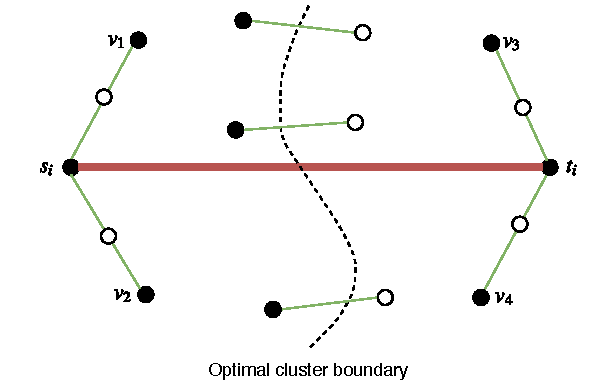
\includegraphics{./img/multicut-multipartite.pdf}
% \caption{Instance of Problem 3 with $|V| + |E|$ vertices}
% \label{fig:5}
% \end{figure}

\section{Problem 4 as hard as multicut}

\begin{theorem}
There can't be an $(\alpha, \alpha)$ bi-criterion approximation to $m$-Robust Correlation Clustering problem if it's NP-hard to $\alpha$-approximate Multicut Problem.
%On a general graph, there exists an approximation preserving reduction from multicut problem to the $m$-Robust Correlation Clustering problem.
\end{theorem}
\begin{proof}
Recall that the aim is to get a bi-criterion approximation in terms of vertices deleted and optimal cost on removing the vertices. We show hardness both in terms of approximating the budget of number of vertices to remove ($\le m$ vertices), and on the optimal cost after removing $m$ vertices.
\end{proof}

\begin{lemma}\label{bi-criterion-hardness-01}
There exists an approximation preserving reduction from unweighted multicut problem on a general graph to finding optimal clustering cost on removing any $m$ vertices.
\end{lemma}
\begin{proof}
\textbf{Construction of problem instance:} Consider a simple undirected graph $G$ of representing an instance of the Multicut problem, with $k$ source-sink pairs $\{ (s_i,t_i), i =1,2,\dots,k \}$. For each pair $(s_i,t_i)$, introduce $n^3$ new vertices, say $v_1^i,v_2^i,\cdots, v_{n^3}^i$. Connect $s_i$ and $t_i$ with $v_1^i,v_2^i,\cdots, v_{n^3}^i$, such that the edge $(s_i,v_j)$ is labelled $+$, and the edge $(t_i,v_j)$ is labelled $-$. Let us also add $m$ more vertices, $\{ u_1,u_2,\dots,u_m \}$, and connect each $u_i$ with each vertex in $G$ in the following way. Consider vertex $q \in V(G)$
\begin{enumerate}
    \item Introduce $n^3$ new vertices, say, $l_1,l_2,\cdots, l_{n^3}$ for each $u_i$, and $q$, and connect such that the edge $q,l_j$ is marked $+1$, and the edge $u_i,l_j$ is marked $-1$.
    \item Introduce $n^3$ more vertices, say, $p_1,p_2,\cdots,p_{n^3}$, for each $u_i$, and $q$, and connect both $q,p_j$ and $u_i,p_j$ through $+1$ marked edge.
\end{enumerate}
The above construction introduces $n^3$ points for each $s_i,t_i$ pair, and $2n^3$ points for each $u_i, q$ pair.

\textbf{Analysis:} Consider the vertex $q$ and $u_i$:
\begin{enumerate}
    \item If both the vertices are in same cluster, the cost is high due to vertices $l_k(s)$, irrespective where we cluster these $l_k(s)$.
    \item If we don't keep $q$ and $u_i$ in same cluster, then cost is very high due to vertices $p_j(s)$.
\end{enumerate}
Hence to construct most optimal clustering after removing any of $m$ vertices of this newly constructed graph, the best strategy would be to remove the vertices $u_1,u_2,\cdots,u_m$ as they add very highly to the cost irrespective of where we place them. And after removing these, the optimal cost of the graph is same as the multicut optimal cost of graph $G$.

\end{proof}
% We first show the hardness in terms of approximating the cost for any $m$ (refer $\ref{IP:CC4}$).
% Consider an undirected simple graph instance $G$ of Multicut problem with $k$ source-sink pairs represented as $(s_i,t_i)$. Connect each $s_i,t_i$ with $v_1,v_2,\cdots, v_{n^3}$, such that the edge $s_i,v_j$ is marked $+1$, and the edge $t_i,v_j$ is marked $-1$. Now add $m$ more vertices, say $u_1,u_2,\cdots,u_m$, and connect each $u_i$ with each vertices in $G$ in the following way:\\
% Let's consider the vertex $q\in V(G)$
% \begin{enumerate}
%     \item Make similar connections like $l_1,l_2,\cdots, l_{n^3}$ between $u_i$, and $q$ such that the edge $q,l_j$ is marked $+1$, and the edge $u_i,l_j$ is marked $-1$.
%     \item Also make similar connections, say $p_1,p_2,\cdots,p_{n^3}$, and mark both the edges $q,p_j$ and $u_i,p_j$ as $+1$.
% \end{enumerate}
% \begin{proof}
% Consider the vertex $q$ and $u_i$:
% \begin{enumerate}
%     \item If they are in same cluster, the cost is high due to vertices $l_k(s)$, irrespective where we cluster these $l_k(s)$.
%     \item If we don't put $q$ and $u_i$ in same cluster, then cost is very high due to vertices $p_j(s)$.
% \end{enumerate}
% Hence, if asked to calculate the most optimal cost possible after removing any of $m$ vertices of this newly constructed graph, the best strategy would be to remove the vertices $u_1,u_2,\cdots,u_m$ as they add very highly to the cost irrespective of where we place them. And after removing these, the optimal cost of the graph is same as the multicut optimal cost of graph $G$.
% \end{proof}

Now we show hardness in terms of approximating $\sum_u Y_u^*$ (refer \ref{IP:CC4}). Consider an undirected simple graph $G=(V,E)$. Also let there be $k$ $s_i\in V,t_i\in V$ source-sink pairs. Define the problem $\vmc$ as of finding minimum number of vertices so that each source-sink pair don't lie in the same connected component.
\begin{lemma}\label{bi-criterion-hardness-02}
There exists an approximation preserving reduction from the $MultiCut$ problem to $\vmc$ problem
%The problem $\vmc$ is as hard as $MultiCut$ problem.
\end{lemma}
\begin{proof}

The idea is to reduce Multicut problem instance on graph $G$ to a $\vmc$ problem instance $I=(V',E')$. Consider the graph $G=(V,E)$ as defined above. Reduce each vertex into a clique of large size, say $n^3$, where $n=|V|$. So there are $n\times n^3$ vertices in instance $I$ with $v_{1}, v_{2}, \dots, v_{n^3}$ representing the clique associated with the vertex $v \in V$. For every $s_i,t_i$ source-sink pair in graph $G$, let each of $s_{i_a}, t_{i_b} \; \forall 1\leq a,b \leq n^3 $ be a source sink pair in instance $I$. So the instance $I$ will now contain $kn^6$ pairs of source-sink compared to only $k$ pairs in graph $G$.

\noindent Let $u,v$ be an edge in graph $G$. Then correspondingly select one of the vertex each from $n^3$ vertices in $u_{1}, u_{2}, \dots, u_{n^3}$ and $v_{1}, v_{2}, \dots, v_{n^3}$, and make an edge between them, say $u_i,v_j$, with the condition that for any vertex $u_{i}$ there should be only one edge of type $u_i, w_j, w\in V$. Basically, there won't be two edges $u_i,v_j$ and $u_i,w_k$ in instance $I$, where $u,v \in E$ and $u,w \in E$.

\noindent We now have a $\vmc$ problem instance $I$. We claim that the reduction from $G$ to $I$ is an approximation preserving reduction. The claim is easy to see. Consider $R$ represent the optimal solution to problem instance $I$, i.e, $R$ contains the optimal set of vertices to remove. Let $u_i\in R$. Removing the edge associated with $u$ corresponding to $u_i$ has similar effect as of removing the vertex $u_i$ in $I$. Removing the path from $u$ to $v$ through removing the edge $u,v$ is achieved by removing the vertex $u_i$ in problem instance $I$. Hence solving the $\vmc$ problem will solve Multicut problem as well
\end{proof}

\begin{lemma}\label{bi-criterion-hardness-03}
There exists an approximation preserving reduction from $\vmc$ problem to approximating on the budget on number of vertices to remove in $m$-Robust Correlation Clustering problem.
\end{lemma}
\begin{proof}
The proof is straightforward. The optimal cost after removing $m$ vertices in above constructed $\vmc$ problem instance is $0$. Basically, the number of vertices to remove on the same problem instance $I$ to make cost $=0$ in $m$-Robust Correlation Clustering is same as computing the optimal vertex set $R$ to be removed in $\vmc$ problem, which is same as finding the optimal number of edges to remove in Multicut problem instance on graph $G$. Therefor from Lemma \ref{bi-criterion-hardness-02} and Lemma \ref{bi-criterion-hardness-03}, $\alpha$-approximating on the budget on number of vertices to remove is not possible if it's NP-hard to $\alpha$-approximate the Multicut problem.
\end{proof}